%versi 3 (22-07-2020)
\chapter{Landasan Teori}
\label{chap:teori}

\section{Portal Akademik Mahasiswa 2018}
\label{sec:pam} 
Portal Akademik Mahasiswa (selanjutnya disingkat dengan PAM) adalah sebuah \textit{web} yang di peruntukan bagi mahasiswa dalam rangka mendapatkan informasi kegiatan akademik mulai dari registrasi, melihat jadwal kuliah dan ujian, info nilai sampai pendaftaran sidang\cite{portalunpar}. Portal Akademik Mahasiswa dapat diakses melalui \url{https://studentportal.unpar.ac.id/}. 

\begin{figure}[H]
	\centering
	
\includegraphics[scale=0.4]{Gambar/halaman2018.jpg}
	\caption{Tampilan halaman awal Portal Akademik Mahasiswa} 
	\label{fig:studpor_home_2018}
\end{figure}

Pada Gambar \ref{fig:studpor_home_2018} adalah tampilan awal ketika masuk ke halaman \url{https://studentportal.unpar.ac.id/}. Mahasiswa perlu melakukan \textit{login} dengan \textit{email} dan \textit{password} mahasiswa UNPAR untuk dapat menggunakan fitur-fitur yang tersedia seperti:
\begin{enumerate}
	\item Fitur mengisi form rencana semester (FRS) atau melakukan perubahan rencana studi (PRS) secara online \\
	Panduan untuk melakukan FRS/PRS online.
	\begin{enumerate}
		\item Masuk ke halaman \url{https://studentportal.unpar.ac.id/} lalu klik tombol ``\textit{Login}'' yang dapat dilihat pada Gambar \ref{fig:studpor_home_2018}.
		\item Lakukan ``\textit{Login}'' dengan memasukan email dan password mahasiswa UNPAR pada halaman sso.
		\begin{figure}[H]
			\centering
			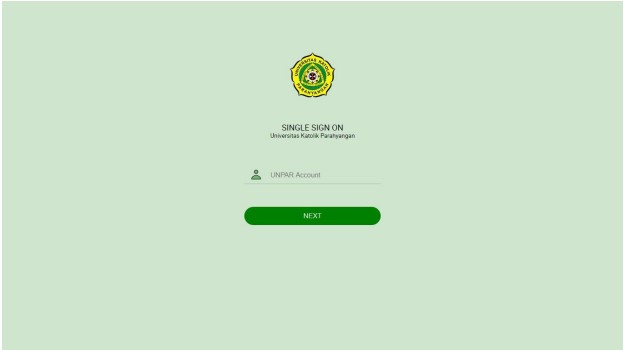
\includegraphics[scale=0.7]{Gambar/sso2018.jpg}
			\caption{Tampilan halaman untuk memasukan \textit{email} Portal Akademik Mahasiswa} 
			\label{fig:sso_2018}
		\end{figure}
	
		\begin{figure}[H]
			\centering
			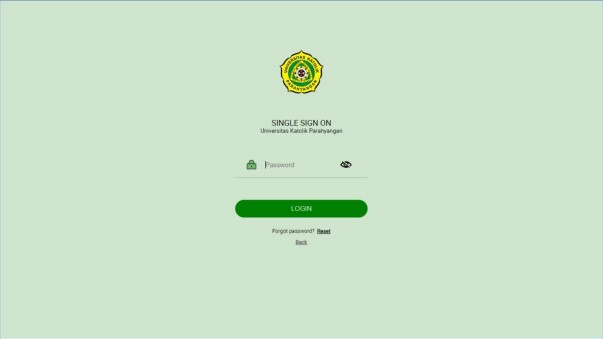
\includegraphics[scale=0.7]{Gambar/pass2018.jpg}
			\caption{Tampilan halaman untuk memasukan \textit{password} Portal Akademik Mahasiswa} 
			\label{fig:pass_2018}
		\end{figure}
		\item Ketika \textit{login} telah berhasil, maka browser akan menampilkan halaman utama, lalu klik pada heksagon berlabel `FRS/PRS' untuk melakukan FRS/PRS online.
		\begin{figure}[H]
			\centering
			
\includegraphics[scale=0.7]{Gambar/frs2018.jpg}
			\caption{Tampilan halaman setelah berhasil \textit{login}} 
			\label{fig:frs_2018}
		\end{figure}
		\item Mahasiswa dapat melakukan FRS sesuai waktu yang sudah ditentukan atau mahasiswa dapat melakukan PRS setelah FRS selesai dan sesuai waktu yang sudah ditentukan untuk PRS.		
	\end{enumerate}
	
	\item Fitur Profil Mahasiswa
	Panduan untuk melihat profil mahasiswa.
	 \begin{enumerate}
	 	\item Mahasiswa melakukan \textit{login} terlebih dahulu. 
	 	\item Menekan menu ``PROFIL'' pada halaman setelah berhasil login seperti pada Gambar \ref{fig:frs_2018}. 
	 	\item Mahasiswa dapat melihat informasi data diri di halaman profil mahasiswa.
	 	\begin{figure}[H]
	 		\centering
	 		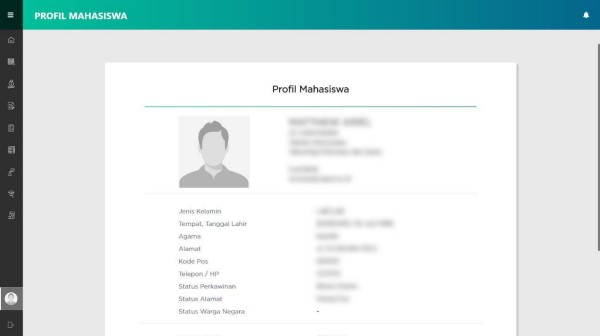
\includegraphics[scale=0.7]{Gambar/profil2018.jpg}
	 		\caption{Tampilan halaman profil mahasiswa} 
	 		\label{fig:profil_2018}
	 	\end{figure}
 	\end{enumerate}
 
	\item Fitur Pembayaran
	Panduan untuk melihat informasi pembayaran.
	\begin{enumerate}
		\item Mahasiswa melakukan \textit{login} terlebih dahulu. 
		\item Menekan menu ``PEMBAYARAN'' pada halaman setelah berhasil login seperti pada Gambar \ref{fig:frs_2018}. 
		\item Pada halaman pembayaran, mahasiswa dapat melihat informasi pembayaran yang terdiri dari Tagihan Pembayaran, Riwayat Pembayaran, dan Keterangan.
	\end{enumerate}
	Pada Gambar \ref{fig:bayar_2018} adalah tabel ``Tagihan Pembayaran'' yang menampilkan jenis tagihan dan jumlah tagihan dari setiap jenis tagihan yang ada.
	\begin{figure}[H]
		\centering
		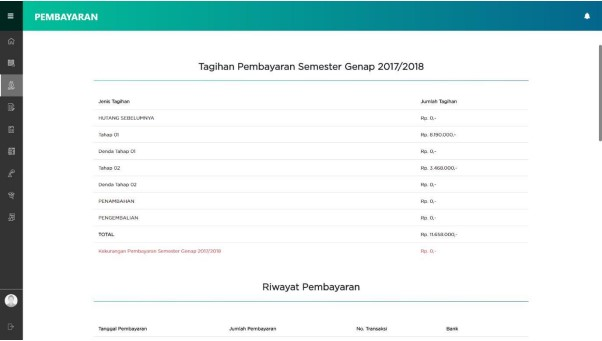
\includegraphics[scale=0.7]{Gambar/bayar2018.jpg}
		\caption{Tampilan halaman pembayaran bagian Tagihan Pembayaran} 
		\label{fig:bayar_2018}
	\end{figure}
	
	Pada Gambar \ref{fig:riw_2018} adalah tabel ``Riwayat Pembayaran'' yang menampilkan histori pembayaran yang telah dilakukan.
	\begin{figure}[H]
		\centering
		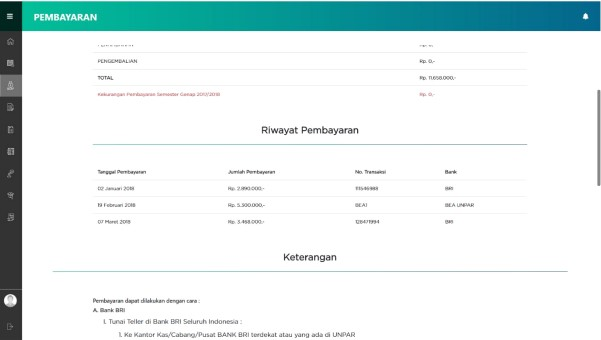
\includegraphics[scale=0.7]{Gambar/riwayat2018.jpg}
		\caption{Tampilan halaman pembayaran bagian Riwayat Pembayaran} 
		\label{fig:riw_2018}
	\end{figure}
	
	Pada Gambar \ref{fig:ketbayar_2018} adalah tabel ``Keterangan'' yang menampilkan tata cara pembayaran yang dapat dilakukan untuk melakukan pembayaran.
	\begin{figure}[H]
		\centering
		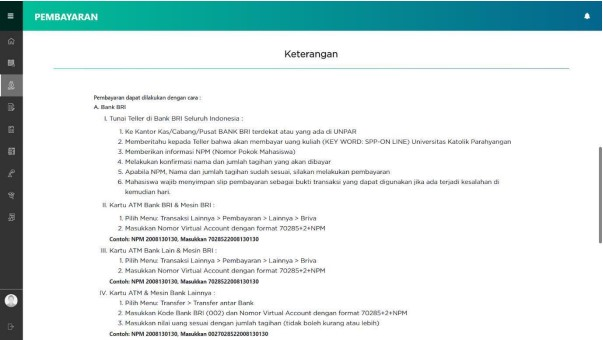
\includegraphics[scale=0.7]{Gambar/keterangan2018.jpg}
		\caption{Tampilan halaman pembayaran bagian Keterangan} 
		\label{fig:ketbayar_2018}
	\end{figure}
	\item Fitur Nilai
	Panduan untuk melihat informasi nilai mahasiswa.
	\begin{enumerate}
		\item Mahasiswa melakukan \textit{login} terlebih dahulu. 
		\item Menekan menu ``NILAI'' pada halaman setelah berhasil login seperti pada Gambar \ref{fig:frs_2018}. 
		\item Pada halaman nilai, mahasiswa dapat melihat informasi nilai dari setiap mata kuliah yang diambil.
		\begin{figure}[H]
			\centering
			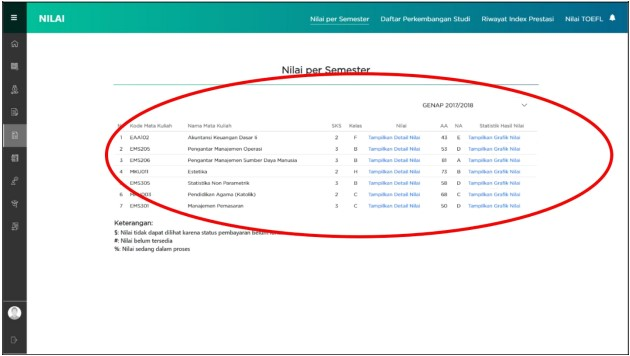
\includegraphics[scale=0.7]{Gambar/nilai2018.jpg}
			\caption{Tampilan halaman nilai bagian Nilai per Semester} 
			\label{fig:nilai_2018}
		\end{figure}
		\item Mahasiswa dapat mengakses menu ``Riwayat Index Prestasi'' untuk melihat `IPK' dan `IPS' mahasiswa.
		\begin{figure}[H]
			\centering
			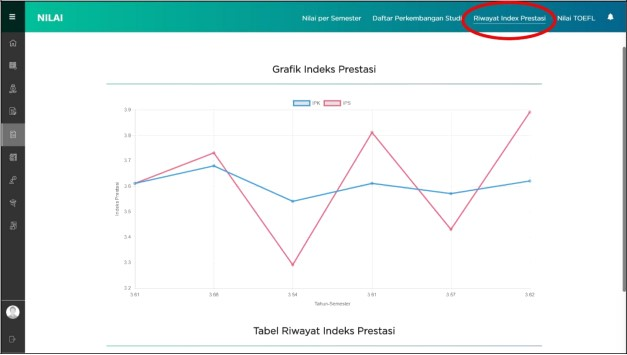
\includegraphics[scale=0.7]{Gambar/rip2018.jpg}
			\caption{Tampilan halaman nilai bagian Riwayat Index Prestasi} 
			\label{fig:rip_2018}
		\end{figure}
	\end{enumerate}	
\end{enumerate}
\newpage

\section{AKUHADIR 2.1}
\label{sec:akuhadir}
\textit{Subbab ini ditulis oleh dosen pembimbing.}

AKUHADIR adalah sebuah portal web yang dibuat bagi pegawai UNPAR dalam melaporkan kehadiran kerja nya secara daring. Pegawai UNPAR mencatatankan kehadirannya setiap hari pada portal tersebut (dapat diakses pada \url{https://akuhadir.unpar.ac.id}), sesuai surat edaran Rektor III/R/2020-07/1153 \cite{akuhadir}.

\begin{figure}[H]
	\centering
	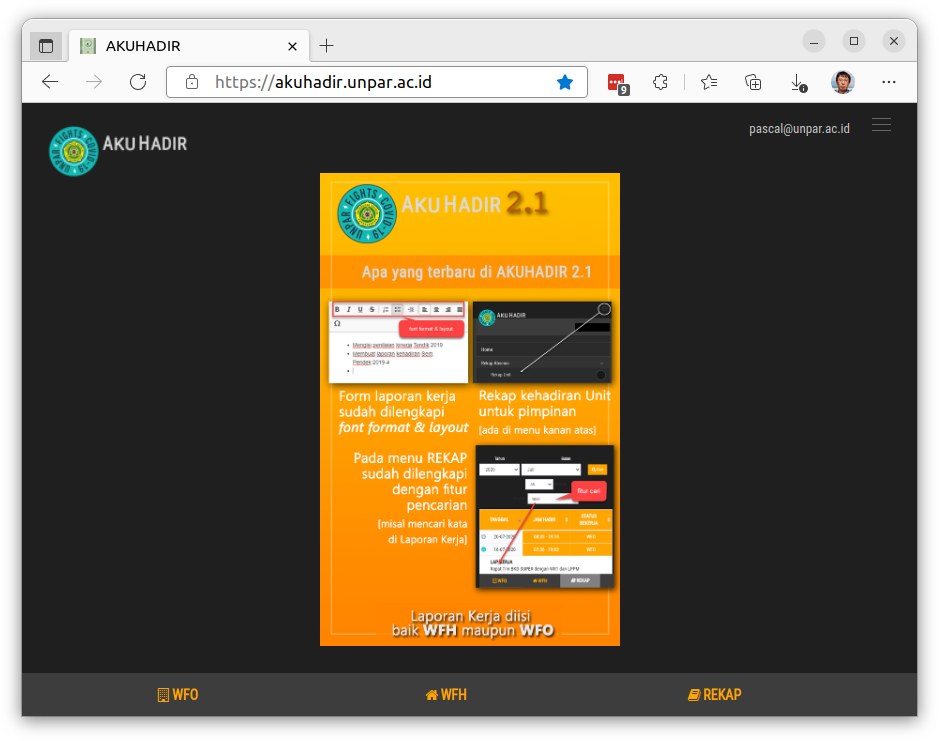
\includegraphics[scale=0.25]{Gambar/akuhadir-1-beranda.png}
	\caption{Tampilan awal halaman AKUHADIR} 
	\label{fig:akuhadir-1-beranda}
\end{figure}

Gambar \ref{fig:akuhadir-1-beranda} menunjukkan halaman awal portal AKUHADIR, setelah pegawai mengautentikasi dirinya melalui SSO (\textit{Single Sign On}) UNPAR. Kehadiran virtual dapat didaftarkan dengan memilih menu WFH di bagian bawah layar, di mana pengguna akan dibawa ke halaman lain yang menunjukkan dua tombol: satu untuk \textit{check in} dan satu untuk \textit{check out} (Gambar \ref{fig:akuhadir-2-wfh}).

\begin{figure}[H]
	\centering
	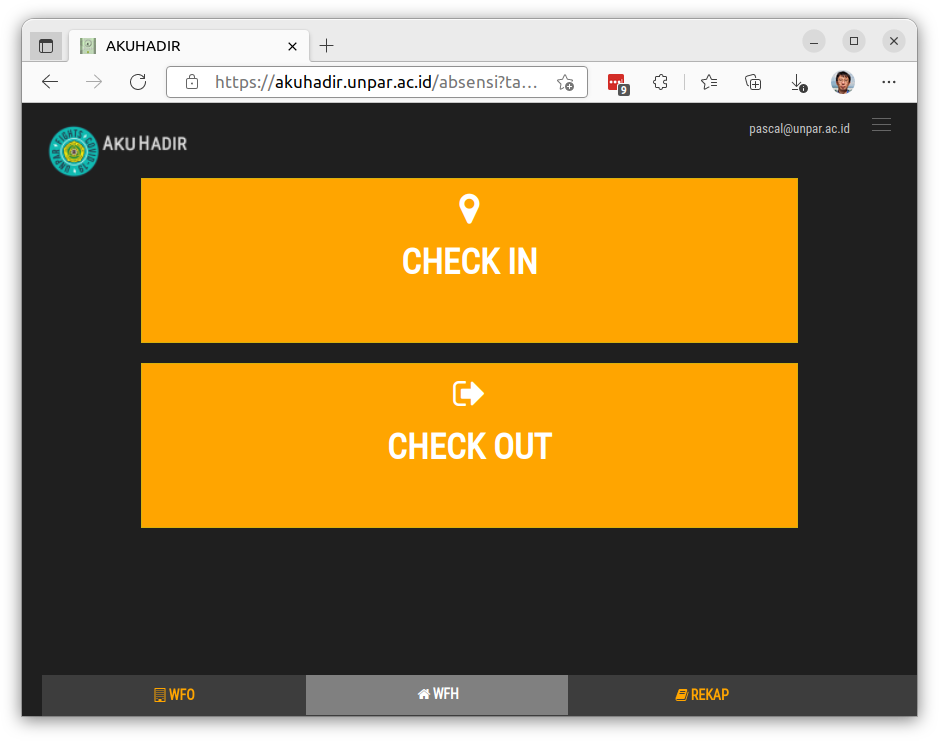
\includegraphics[scale=0.25]{Gambar/akuhadir-2-wfh.png}
	\caption{Tampilan menu WFH} 
	\label{fig:akuhadir-2-wfh}
\end{figure}

Di pagi hari sebelum memulai bekerja, pegawai mengklik menu \textit{Check in}. Setelah tombol tersebut diklik, akan muncul pesan konfirmasi bahwa \textit{check in} sudah berhasil dilakukan (Gambar \ref{fig:akuhadir-3-wfh-checkin}).

\begin{figure}[H]
	\centering
	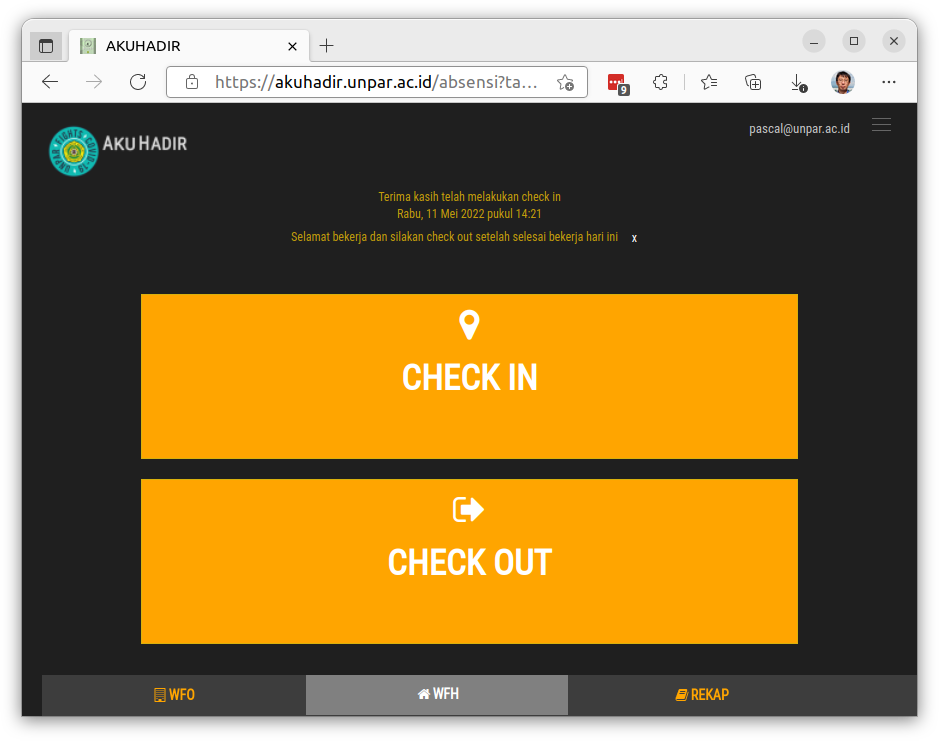
\includegraphics[scale=0.25]{Gambar/akuhadir-3-wfh-checkin.png}
	\caption{Tampilan konfirmasi check in AKUHADIR} 
	\label{fig:akuhadir-3-wfh-checkin}
\end{figure}

Di sore hari setelah bekerja, pegawai kembali mengakses AKUHADIR, namun memilih menu \textit{check out}. Prosesnya mirip dengan \textit{check in}, namun pada proses \textit{check out} pegawai diminta untuk menuliskan laporan pekerjaan yang sudah dilakukan pada hari tersebut dalam bentuk tulisan (Gambar \ref{fig:akuhadir-4-wfh-checkout}).

\begin{figure}[H]
	\centering
	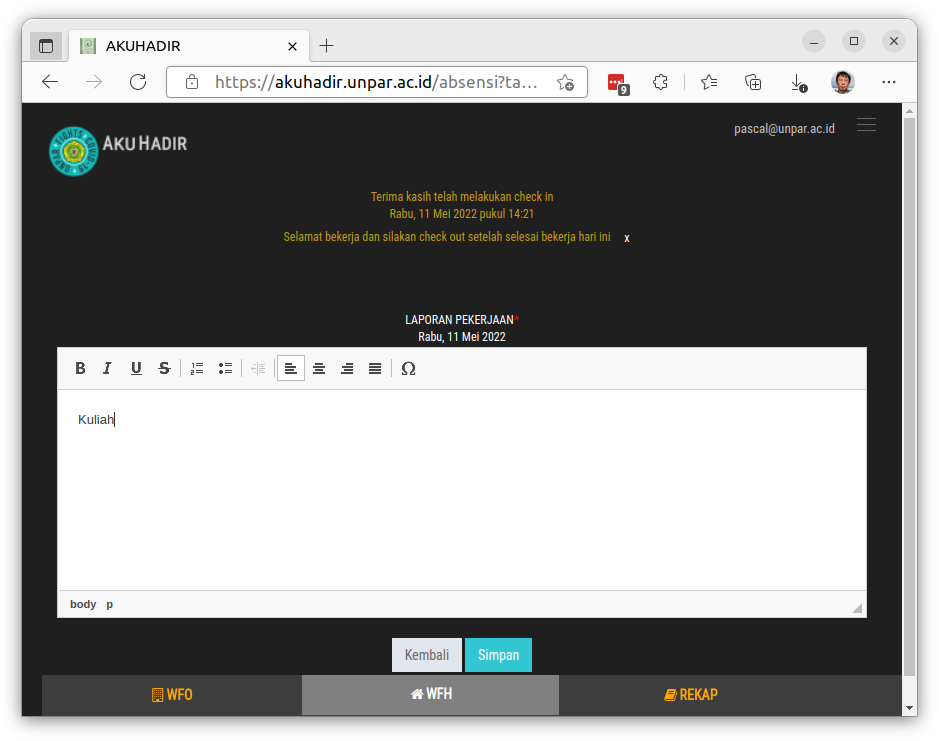
\includegraphics[scale=0.25]{Gambar/akuhadir-4-wfh-checkout.png}
	\caption{Tampilan halaman check out AKUHADIR} 
	\label{fig:akuhadir-4-wfh-checkout}
\end{figure}

Selain kedua fitur tersebut, ada beberapa fitur lain dari AKUHADIR yang tidak dijelaskan lebih mendalam di sini karena tidak terkait erat dengan penelitian yang dilakukan:

\begin{itemize}
	\item \textbf{WFO} untuk melihat status pelaporan bekerja dari kantor (pelaporan bekerja dari kantor dilakukan oleh petugas keamanan UNPAR yang memindai kode batang pegawai).
	\item \textbf{Rekap} untuk melihat rekapitulasi pelaporan bekerja, baik WFH maupun WFO.
	\item \textbf{Profil} untuk menampilkan foto serta kode batang pegawai. Bisa digunakan untuk menunjukkan kode batang kepada petugas keamanan dalam rangka pelaporan WFO.
	\item \textbf{About} saat ini hanya menampilkan informasi versi dan \textit{copyright}.
\end{itemize}

\section{\textit{Cascading Style Sheets} (CSS) \textit{Selector}}
\label{sec:css}
\textit{Cascading Style Sheets} (CSS) adalah bahasa untuk menerapkan tampilan pada sebuah halaman web, hal tersebut termasuk tata letak, warna, dan \textit{font}\cite{css}. CSS sudah menjadi bagian penting untuk sebuah Web. CSS \textit{Selector} digunakan untuk menemukan atau memilih elemen HTML yang diinginkan berdasarkan \textit{style} CSS\footnote{\textit{CSS Selector} \url{https://www.w3schools.com/css/css_selectors.asp}}. Terdapat lima kategori pada CSS \textit{Selector}:
\begin{enumerate}
	\item \textit{Simple selectors} merupakan pemilihan elemen dari CSS berdasarkan \textit{name}, id, dan \textit{class}. Pada Tabel \ref{table:simpel} merupakan contoh cara mengambil elemen menggunakan cara \textit{simple selector}.
		\begin{table}[h!]
			\centering
			\caption{Tabel Contoh \textit{Simple Selector}.}
			\label{table:simpel}
			\begin{tabular}{ | m{8em} | m{3cm}| m{8cm} | } 
				\hline
				\textit{\textbf{Selector}}& Contoh & Penjelasan \\ 
				\hline
				\#id & 	\#firstname & Memilih elemen dengan id = ``firstname''. \\ 
				\hline
				.class & .intro & Memilih elemen dengan \textit{class} = ``intro''. \\ 
				\hline
				element & p & Memilih semua elemen <p>. \\ 
				\hline
				* & * & Memilih semua elemen.  \\ 
				\hline
				element.class & p.intro & Memilih hanya elemen <p> pada class = ``intro''.  \\ 
				\hline
			\end{tabular}
		\end{table}
	\item \textit{Combinator selectors} merupakan pemilihan elemen dari CSS berdasarkan gabungan atau kombinasi antar elemen pada CSS. Pada Tabel \ref{table:combinator} merupakan contoh cara mengambil elemen menggunakan cara \textit{combinator selector}.
		\begin{table}[h!]
			\centering
			\caption{Tabel Contoh \textit{Combinator Selector}.}
			\label{table:combinator}
			\begin{tabular}{ | m{9em} | m{2cm}| m{8cm} | } 
				\hline
				\textit{\textbf{Selector}}& Contoh & Penjelasan \\ 
				\hline
				element element & div p & Memilih semua elemen <p> yang berada di dalam elemen <div>. \\ 
				\hline
				element > element & div > p & Memilih semua elemen <p> yang menjadi anak bagian elemen <div>. \\ 
				\hline
				element + element & div + p & Memilih elemen <p> pertama setelah elemen <div>. \\ 
				\hline
				element1 $\sim$ element2 & p $\sim$ ul & Memilih setiap elemen <ul> yang diawali dulu oleh elemen <p>.  \\ 
				\hline
			\end{tabular}
		\end{table}
	\item \textit{Pseudo-class selectors} merupakan pemilihan elemen yang berada dalam kondisi khusus elemen tersebut. Penjelasan lebih detail dapat dilihat pada Tabel \ref{table:pclass} merupakan contoh cara mengambil elemen menggunakan cara \textit{pseudo-class selector}. 
		\begin{table}[h!]
			\centering
			\caption{Tabel Contoh \textit{Pseudo-class Selector}.}
			\label{table:pclass}
			\begin{tabular}{ | m{8em} | m{3cm}| m{8cm} | } 
				\hline
				\textit{\textbf{Selector}}& Contoh & Penjelasan \\ 
				\hline
				:active & a:active & Memilih elemen yang memiliki link aktif. \\ 
				\hline
				:checked & input:checked & Memilih setiap elemen <input> yang sudah ditandai. \\ 
				\hline
				:disabled & input:disabled & Memilih setiap elemen <input> yang dinonaktifkan. \\ 
				\hline
			\end{tabular}
		\end{table}
	\item \textit{Pseudo-elements selectors } merupakan pemilih elemen berdasarkan pada letak spesifik elemen tersebut berada. Pada Tabel \ref{table:pelemen} merupakan contoh cara mengambil elemen menggunakan cara \textit{pseudo-elements selector}.
		\begin{table}[h!]
			\centering
			\caption{Tabel Contoh \textit{Pseudo-elements Selector}.}
			\label{table:pelemen}
			\begin{tabular}{ | m{8em} | m{3cm}| m{8cm} | } 
				\hline
				\textit{\textbf{Selector}}& Contoh & Penjelasan \\ 
				\hline
				::first-letter & p::first-letter & Memilih huruf pertama dari setiap elemen <p>. \\ 
				\hline
				::first-line & p::first-line & Memilih baris pertama dari setiap elemen <p>. \\ 
				\hline
			\end{tabular}
		\end{table}
	\item \textit{Attribute selectors} merupakan pemilihan elemen berdasarkan atribut tertentu atau nilai dari atributnya. Pada Tabel \ref{table:attribut} merupakan contoh cara mengambil elemen menggunakan cara \textit{attribute selector}.
		\begin{table}[h!]
			\centering
			\caption{Tabel Contoh \textit{Attribute Selector}.}
			\label{table:attribut}
			\begin{tabular}{ | m{8em} | m{3cm}| m{8cm} | } 
				\hline
				\textit{\textbf{Selector}}& Contoh & Penjelasan \\ 
				\hline
				[attribute] & [target] & Memilih semua elemen yang mengandung atribut ``target''.  \\ 
				\hline
				[attribute=value] & [target=blank] & Memilih semua elemen yang mengandung atribut ``target'' yang nilainya ``blank''. \\ 
				\hline
				[attribute~=value] & [title~=flower] & Memilih semua elemen yang ``title'' atributnya mengandung kata ``flower''.\\ 
				\hline
			\end{tabular}
		\end{table}
\end{enumerate}


\section{Selenium}
\label{sec:selenium}
Selenium merupakan \textit{open-source} \textit{framework} untuk pengujian otomatisasi untuk browser web\cite{selenium}. Cara kerja Selenium untuk melakukan otomatisasi pada browser web adalah seperti menirukan interaksi pengguna dengan browser, yang nantinya akan dijalankan otomatis oleh Selenium. Otomatisasi dengan Selenium ini dapat dilakukan pada berbagai browser yang umum banyak digunakan (Google Chrome, Safari, Opera, Firefox). Selenium ini tersedia untuk bahasa pemrograman Ruby, Java, Python, C\#, dan JavaScript. Bagian inti dari Selenium adalah WebDriver, WebDriver merupakan sebuah \textit{interface} untuk menulis suatu instruksi yang dapat dijalankan secara otomatis dan bergantian pada \textit{browser}. Setiap browser pasti didukung oleh implementasi WebDriver tertentu, yang disebut driver. Driver adalah komponen yang bertanggung jawab untuk menghubungkan komunikasi antara Selenium dengan browser. 
\begin{figure}[H]
	\centering
	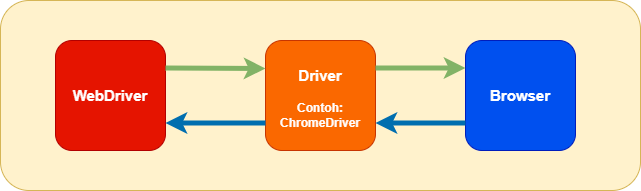
\includegraphics[scale=0.7]{Gambar/flowSelenium.png}
	\caption{Alur Komunikasi WebDriver dengan Browser} 
	\label{fig:flowSelenium}
\end{figure}
Pada Gambar \ref{fig:flowSelenium}. Pada Gambar \ref{fig:flowSelenium} ini komunikasi WebDriver yang merupakan bagian dari Selenium memberikan perintah kepada browser melalui \textit{driver} browser tersebut dan menerima hasil informasinya kembali melalui alur yang sama.

\section{WebDriver}
\label{sec:webdriver}
WebDriver adalah \textit{Application Programming Interface} (API) yang berfungsi menghubungkan Selenium dengan browser web, sehingga Selenium dapat mengontrol atau melakukan otomatisasi pada browser web\cite{selenium}. API WebDriver ini seolah-olah membuat pengguna secara langsung mengoperasi \textit{browser}, padahal dijalankan secara otomatis langsung oleh API WebDriver tersebut. 
\textit{Driver} browser adalah komponen yang bertanggung jawab untuk menghubungkan antara Selenium dengan browser agar dapat dikendalikan. Driver browser yang tersedia untuk selenium adalah Google Chrome, Firefox, Edge, Internet Explorer, dan Safari. Agar browser dapat dibuka untuk melakukan otomatisasi, maka perlu melakukan \textit{install} driver dari browser yang ingin digunakan. Pada subbab ini dijelaskan bagian dari WebDriver yang digunakan untuk pembuatan program perekaman kehadiran daring otomatis.

\subsection{Browser}
Selenium Webdriver dapat mengambil informasi mengenai browser yang sedang dibuka. Informasi yang dapat diambil adalah judul dari situs web yang sedang dibuka pada browser (Kode \ref{kode:2:getinfo} baris 1) dan mendapatkan alamat situs web yang sedang dibuka (Kode \ref{kode:2:getinfo} baris 2). 
\begin{lstlisting}[language=python, caption=Contoh Potongan Kode \textit{Get Title} dan \textit{Get Current URL}, label=kode:2:getinfo]
	driver.title
	driver.current_url
\end{lstlisting}
Hal pertama yang perlu dilakukan setelah berhasil membuka browser adalah membuka situs web yang akan diotomatisasikan. Pada Kode \ref{kode:2:navigate} merupakan contoh untuk memunculkan situs web yang ingin dijalankan dengan selenium. Baris 1 melakukan \textit{import} webdriver terlebih dahulu, lalu baris 2 \textit{string} dengan nama driver memanggil webdriver yang ingin digunakan, yaitu Google Chrome dan diisi letak file chromedriver.exe disimpan. Baris 3 \textit{string} dengan nama url diisi dengan situs web yang dituju dalam contoh adalah \url{https://selenium.dev}. Baris 4 adalah \textit{string} dengan nama link menggunakan \textit{method get} yang memanggil \textit{string} dengan nama driver yang sudah memanggil webdriver, lalu ditambahkan \textit{method get} yang memanggil \textit{string} dengan nama url yang sudah berisi situs web yang dituju.
	\begin{lstlisting}[language=python, caption=Contoh kode Navigate to, label=kode:2:navigate]
		from selenium import webdriver
		driver = webdriver.Chrome()
		url = "https://selenium.dev"
		link = driver.get(url)
	\end{lstlisting}
WebDriver juga dapat melakukan otomatisasi untuk keluar dari browser setelah selesai digunakan. Pada Kode \ref{kode:2:quit} merupakan contoh untuk dapat keluar dari \textit{browser} setelah selesai menggunakan. Pada baris 1 sampai 4 merupakan contoh untuk memunculkan situs web yang ingin dijalankan dengan selenium dan sudah dijelaskan pada Kode \ref{kode:2:navigate}. Baris 5 adalah \textit{string} dengan nama \textit{quit} yang memanggil \textit{method quit()} yang berfungsi untuk dapat keluar dari \textit{browser} setelah selesai digunakan.
\newpage
	\begin{lstlisting}[language=python, caption=Contoh kode Get title, label=kode:2:quit]
		from selenium import webdriver
		driver = webdriver.Chrome()
		url = "https://selenium.dev"
		link = driver.get(url)
		quit = driver.quit()
	\end{lstlisting}

\subsection{Menemukan elemen}
Salah satu teknik mendasar untuk dipelajari saat menggunakan WebDriver adalah cara menemukan elemen di halaman web. WebDriver menyediakan berbagai cara untuk menemukan elemen, terdapat delapan cara menemukan elemen:
\begin{itemize}
	\item Id \\
	Menemukan elemen yang atribut ID-nya cocok dengan nilai pencarian. Pada Kode \ref{kode:2:elemenid} merupakan contoh untuk menemukan elemen dengan atribut ID. Baris 1 melakukan \textit{import} webdriver terlebih dahulu. Baris 2 melakukan \textit{import} By yang merupakan \textit{library} yang sudah ada milik selenium untuk digunakan dalam menemukan elemen. lalu baris 3 \textit{string} dengan nama driver memanggil webdriver yang ingin digunakan, yaitu Google Chrome untuk membuka browsernya. Baris 4 \textit{string} dengan nama url diisi dengan situs web yang dituju dalam contoh adalah \url{https://selenium.dev}. Baris 5 adalah \textit{string} dengan nama link menggunakan \textit{method get} yang memanggil \textit{string} dengan nama driver yang sudah memanggil webdriver, lalu ditambahkan \textit{method get} yang memanggil \textit{string} dengan nama url yang sudah berisi situs web yang dituju. Baris 6 atau 7 merupakan contoh kode yang dapat digunakan untuk menemukan elemen berdasarkan atribut ID dengan nama id ``selenium'' dari situs web \url{https://selenium.dev}. Kode pada baris 6 dan 7 hanya berbeda cara penulisannya saja. 
	\begin{lstlisting}[language=python, caption=Contoh kode untuk menemukan elemen dengan atribut ID, label=kode:2:elemenid]
		from selenium import webdriver
		from selenium.webdriver.common.by import By
		driver = webdriver.Chrome()
		url = "https://selenium.dev"
		driver.get(url)
		driver.find_element(By.ID, "selenium")	
		driver.find_element_by_id("selenium")
	\end{lstlisting}
	
	\item \textit{Class name}\\
	Menemukan elemen yang nama kelasnya berisi nilai pencarian. Pada Kode \ref{kode:2:elemenclass} merupakan contoh untuk menemukan elemen dengan nama kelas. Pada baris 1 sampai 5 merupakan contoh melakukan \textit{import library} selenium yang dibutuhkan dan untuk memunculkan situs web yang ingin dijalankan dengan selenium dan sudah dijelaskan pada Kode \ref{kode:2:elemenid}. Baris 6 merupakan contoh kode untuk mencari elemen dengan \textit{class name} ``text-center'' dan disimpan dalam \textit{string} kelas.
	\begin{lstlisting}[language=python, caption=Contoh kode untuk menemukan elemen dengan \textit{class name}, label=kode:2:elemenclass]
		from selenium import webdriver
		from selenium.webdriver.common.by import By
		driver = webdriver.Chrome()
		url = "https://selenium.dev"
		driver.get(url)
		kelas = driver.find_elements(By.CLASS_NAME, "text-center")
	\end{lstlisting}

	\item \textit{CSS selector}\\
	Menemukan elemen yang cocok dengan pemilihan \textit{Cascading Style Sheets} (CSS). Pemilihan pada CSS adalah pola yang digunakan untuk memilih elemen dengan \textit{style} yang diinginkan. Pada Kode \ref{kode:2:elemencss} merupakan contoh untuk menemukan elemen yang cocok dengan pemilihan CSS. Baris 6 merupakan contoh kode yang disimpan dalam \textit{string} \textit{select} untuk mencari elemen berdasarkan pemilihan CSS dengan mengambil elemen dengan id ``selenium\_logo''.
	\begin{lstlisting}[language=python, caption=Contoh kode untuk menemukan elemen dengan \textit{CSS selector}, label=kode:2:elemencss]
		from selenium import webdriver
		from selenium.webdriver.common.by import By
		driver = webdriver.Chrome()
		url = "https://selenium.dev"
		driver.get(url)
		select = driver.find_element(By.CSS_SELECTOR,"#selenium_logo")
	\end{lstlisting}

	\item \textit{Name}\\
	Menemukan elemen yang atribut \textit{name} yang cocok dengan nilai pencarian. Pada Kode \ref{kode:2:elemenname} baris 6 mencari elemen dari atribut namanya dari situs web \url{https://www.facebook.com/} dengan atribut namanya adalah ``email'' dan disimpan dalam \textit{string} nama.
	\begin{lstlisting}[language=python, caption=Contoh kode untuk menemukan elemen dengan atribut nama, label=kode:2:elemenname]
		from selenium import webdriver
		from selenium.webdriver.common.by import By
		driver = webdriver.Chrome()
		url = "https://www.facebook.com/"
		driver.get(url)
		nama = driver.find_element(By.NAME,"email")
	\end{lstlisting}

	\item Link text\\
	Menemukan elemen \textit{link} yang teksnya terlihat cocok dengan nilai pencarian. Pada Kode \ref{kode:2:elemenlink} baris 6 mencari elemen \textit{link} yang dengan nama teksnya adalah ``Documentation'' dari situs web \url{https://selenium.dev}.
	\begin{lstlisting}[language=python, caption=Contoh kode untuk menemukan elemen dengan \textit{link text}, label=kode:2:elemenlink]
		from selenium import webdriver
		from selenium.webdriver.common.by import By
		driver = webdriver.Chrome()
		url = "https://selenium.dev"
		driver.get(url)
		nama = driver.find_element(By.LINK_TEXT, "Documentation")
	\end{lstlisting}

	\item Partial link text\\
	Menemukan elemen \textit{link} yang teksnya terlihat berisi nilai pencarian. Jika beberapa elemen cocok, hanya yang pertama yang akan dipilih. Pada Kode \ref{kode:2:elemenpartial} baris 6 mencari elemen \textit{link} yang dengan nama teksnya adalah ``About Selenium'' dari situs web \url{https://selenium.dev}, namun ketika ada beberapa elemen yang cocok dengan nama teks yang dicari maka akan diambil yang pertamanya saja.
	\begin{lstlisting}[language=python, caption=Contoh kode untuk menemukan elemen dengan \textit{partial link text}, label=kode:2:elemenpartial]
		from selenium import webdriver
		from selenium.webdriver.common.by import By
		driver = webdriver.Chrome()
		url = "https://selenium.dev"
		driver.get(url)
		nama = driver.find_element(By.PARTIAL_LINK_TEXT, "About Selenium")
	\end{lstlisting}
	
	\item Tag name\\
	Menemukan elemen yang nama tagnya cocok dengan nilai pencarian. Pada Kode \ref{kode:2:elementag} baris 6 mencari elemen yang nama tagnya adalah ``h1'' dari situs web \url{https://selenium.dev} yang disimpan dengan \textit{string} \textit{tag}.
	\begin{lstlisting}[language=python, caption=Contoh kode untuk menemukan elemen dengan \textit{tag name}, label=kode:2:elementag]
		from selenium import webdriver
		from selenium.webdriver.common.by import By
		driver = webdriver.Chrome()
		url = "https://selenium.dev"
		driver.get(url)
		tag = driver.find_element(By.TAG_NAME, "h1")
	\end{lstlisting}
	
	\item XPath\\
	Menemukan elemen yang cocok dengan ekspresi \textit{XML Path Language} (XPath). XPath adalah bahasa ekspresi yang dirancang untuk mendukung kueri atau transformasi dari dokumen XML\cite{xpath}. Pada Kode \ref{kode:2:elemenxpath} baris 6 mencari elemen dengan XPath mulai dari nama id dari element yang dicari adalah `td-cover-block-0', lalu diarahkan hingga tempat elemen yang dicari itu berada, dan disimpan di \textit{string} dengan nama ``contoh1''. Pada baris 7 mencari elemen dengan XPath yang mulai dari struktur webnya dari atas hingga menuju tempat elemen itu berada dan disimpen di \textit{string} dengan nama ``contoh2''.
	\begin{lstlisting}[language=python, caption=Contoh kode untuk menemukan elemen dengan ekspresi XPath, label=kode:2:elemenxpath]
		from selenium import webdriver
		from selenium.webdriver.common.by import By
		driver = webdriver.Chrome()
		url = "https://selenium.dev"
		driver.get(url)
		contoh1 = driver.find_element(By.XPATH, "//*[@id='td-cover-block-0']/div/div/div/div/h1")
		contoh2 = driver.find_element(By.XPATH, "/html/body/div/main/section[1]/div/div/div/div/h1")
	\end{lstlisting}
\end{itemize}

\subsection{Interaksi Elemen}
Interaksi elemen merupakan metode selenium yang dirancang untuk dapat melakukan otomatisasi seperti meniru langsung pengguna dalam melakukan sesuatu pada browser, seperti mengklik tombol, memasukan email dan \textit{password}, atau menghapus teks sesuatu. Terdapat 5 perintah dasar yang dapat dijalankan pada sebuah elemen:
\begin{itemize}
	\item \textit{Click}\\
	Perintah \textit{Click} merupakan perintah dasar milik selenium untuk menekan atau mengklik secara otomatis sesuai dengan elemen yang diambil. Pada Kode \ref{kode:2:elemenclick} adalah contoh potongan kode program yang menggunakan perintah \textit{Click}, hanya cukup menambahkan kode ``.click()'' saja pada bagian akhir saat mengambil suatu elemen.
	\begin{lstlisting}[language=python, caption=Contoh Potongan Kode Perintah \textit{Click} pada Suatu Elemen, label=kode:2:elemenclick]
		btnIn = driver.find_element(By.CSS_SELECTOR, "#login-button").click()
	\end{lstlisting}
	
	\item \textit{Send Keys}\\
	Perintah \textit{Send Keys} merupakan perintah untuk mengetik sesuatu atau memasukan sesuatu dalam bentuk teks maupun angka pada suatu elemen secara otomatis. Biasanya elemen yang digunakan untuk menjalankan perintah \textit{Send Keys} ini adalah elemen input dari formulir pada suatu situs web dengan tipe teks. Pada Kode \ref{kode:2:elemensendkeys} adalah contoh potongan kode program yang menggunakan perintah \textit{Send Keys}, kode tersebut mengartikan bahwa program melakukan pencarian secara otomatis pada situs ``http://www.google.com'', dimana elemen dengan \textit{NAME} ``q'' diisi dengan nilai ``webdriver'' dan menekan tombol ``ENTER'' secara otomatis seperti pengguna menekan tombol ``ENTER'' manual pada \textit{keyboard} komputer atau laptop. Hasilnya adalah program akan membuka situs ``http://www.google.com'' dan sudah melakukan pencarian tentang ``webdriver''.
	\begin{lstlisting}[language=python, caption=Contoh Potongan Kode Perintah \textit{Send Keys} pada Suatu Elemen, label=kode:2:elemensendkeys]
		from selenium import webdriver
		from selenium.webdriver.common.by import By
		from selenium.webdriver.common.keys import Keys
		driver = webdriver.Chrome()
		driver.get("http://www.google.com")
		driver.find_element(By.NAME, "q").send_keys("webdriver" + Keys.ENTER)
	\end{lstlisting}
	
	\item \textit{Clear}\\
	Perintah \textit{Clear} merupakan perintah untuk menghapus secara otomatis terhadap isi konten pada suatu elemen. Elemen yang bisa diberi perintah \textit{Clear} adalah elemen input dari formulir pada suatu situs web dengan tipe teks. Pada Kode \ref{kode:2:elemenclear} adalah contoh potongan kode program yang menggunakan perintah \textit{Clear}, kode tersebut mengartikan bahwa program setelah menggunakan perintah \textit{Send Keys} untuk memasukan ``webdriver'' pada elemen dengan \textit{NAME} ``q'' untuk dicari pada situs ``http://www.google.com''. Lalu dihapus dengan menggunakan perintah \textit{Clear}.
	\begin{lstlisting}[language=python, caption=Contoh Potongan Kode Perintah \textit{Clear} pada Suatu Elemen, label=kode:2:elemenclear]
		from selenium import webdriver
		from selenium.webdriver.common.by import By
		driver = webdriver.Chrome()
		driver.get("http://www.google.com")
		SearchInput = driver.find_element(By.NAME, "q").send_keys("webdriver")
		SearchInput.clear()
	\end{lstlisting}
	
	\item \textit{Submit}\\
	Perintah \textit{Submit} pada Selenium versi 4 saat ini sudah tidak lagi diimplementasikan lagi, sehingga disarankan tidak menggunakan perintah ini lagi dan disarankan menggunakan perintah \textit{Click} dengan memilih elemen yang tepat untuk tombol \textit{submit} pada situs web.
	
	\item \textit{Select List}\\
	Perintah \textit{Select List} ini berfungsi untuk mengambil nilai dari elemen yang berada dalam bentuk \textit{list}.
\end{itemize}

\subsection{Waits}
\textit{Waits} merupakan API pemblokiran yang dimiliki WebDriver. \textit{Waits} ini memiliki fungsi untuk menunggu suatu perintah saat melakukan proses otomatisasi terhadapa suatu situs web beres dijalankan, lalu menjalankan perintah selanjutnya. 
\begin{itemize}
	\item Implicit wait: memberi tahu WebDriver untuk menunggu selama jangka waktu tertentu ketika mencoba menemukan elemen. Pengaturan awal lama menunggunya adalah 0 detik, artinya dinonaktifkan. Setelah disetel, maka \textit{wait implicit} disetel untuk menunggu selama waktu yang sudah ditentukan.
	\begin{lstlisting}[language=python, caption=Contoh kode Implicit wait, label=kode:2:implicit]
		from selenium import webdriver
		from selenium.webdriver.common.by import By
		from selenium.webdriver.support.ui import WebDriverWait
		driver = webdriver.Chrome()
		driver.implicitly_wait(10)
		url = "https://selenium.dev"
		driver.get(url)
		cari = driver.find_element(By.ID, "navbarDropdown")
	\end{lstlisting}
	Pada Kode \ref{kode:2:implicit} merupakan contoh kode \textit{implicit wait} dimana pada baris 1 sampai 3 melakukan \textit{import} library yang diperlukan. Baris 4 untuk menjalankan webdriver Google Chrome. Baris 5 merupakan kode \textit{implicit wait} yang dimana kode tersebut memberikan waktu selama 10 detik untuk menemukan elemen yang ingin dicari. Baris 6 \textit{string} dengan nama ``url'' diisi dengan situs web yang akan dituju. Baris 7 menggunakan \textit{method get} yang memanggil \textit{string} dengan nama ``url'' yang sudah berisi situs web yang dituju. Baris 8 adalah untuk menemukan elemen yang dicari dengan id ``navbarDropdown''. Jika selama waktu yang diberikan tidak dapat menemukan elemen yang dicari maka program akan mengeluarkan \textit{output} bahwa elemen yang dicari tidak ditemukan.
	
	\item Explicit wait: mengizinkan kode untuk menghentikan eksekusi program, atau membekukan \textit{thread}, hingga suatu kondisi dapat teratasi. Kondisi ini dipanggil dengan frekuensi tertentu sampai batas waktu tunggu terlewati.
	\begin{lstlisting}[language=python, caption=Contoh kode Explicit wait, label=kode:2:explicit]
		from selenium import webdriver
		from selenium.webdriver.common.by import By
		from selenium.webdriver.support.ui import WebDriverWait
		from selenium.webdriver.support import expected_conditions as EC
		driver = webdriver.Chrome()
		url = "https://selenium.dev"
		driver.get(url)	
		try:
			element = WebDriverWait(driver, 10).until(
			EC.presence_of_element_located((By.ID, "navbarDropdown"))
			)
		finally:
			driver.quit()
	\end{lstlisting}
	Pada Kode \ref{kode:2:explicit} merupakan contoh kode \textit{explicit wait} dimana pada baris 1 sampai 4 melakukan \textit{import} library yang diperlukan. Baris 5 untuk menjalankan webdriver Google Chrome. Baris 6 \textit{string} dengan nama ``url'' diisi dengan situs web yang akan dituju. Baris 7 menggunakan \textit{method get} yang memanggil \textit{string} dengan nama ``url'' yang sudah berisi situs web yang dituju. Baris berikutnya adalah selenium akan menunggu selama 10 detik untuk menemukan elemen yang sesuai dengan id ``navbarDropdown''. Jika berhasil menemukan elemen yang dicari maka akan langsung masuk kondisi kode finally pada baris 11 dan langsung keluar dari webdriver Google Chrome, Jika tidak ada elemen yang ditemukan selama waktu yang diberikan maka program memberikan \textit{output} \textit{TimeoutException} dan akan masuk ke kode baris 11 serta langsung keluar dari webdriver Google Chrome.	
\end{itemize}

\section{\textit{Library} Python}
\label{sec:library}
Bahasa pemrograman Python memiliki banyak library yang dapat dipakai. \textit{Library} Pyton adalah kumpulan modul yang berisi kumpulan kode yang dapat digunakan secara berulang kali di berbagai program. \textit{Library} Python ini membuat programmer menjadi mudah dan sederhana, karena tidak perlu menuliskan kode yang sama secara berulang. Pada subbab ini dijelaskan \textit{library} python yang digunakan untuk pembuatan program perekaman kehadiran daring otomatis.

\subsection{\textit{Configuration File Parser} (ConfigParser)}
ConfigParser merupakan sebuah modul yang sudah tersedia pada bahasa pemrograman Python dan mengimplementasikan bahasa konfigurasi dasar\cite{parser}. Penggunaan ConfigParser pada bahasa pemrograman python perlu melakukan \textit{import library} terlebih dahulu, sehingga dapat digunakan. Struktur dari file konfigurasi terdiri dari \textit{section} dari file tersebut dan masing-masing \textit{key} dan \textit{value}. ConfigParser ini dapat membaca dan menulis file tersebut. 
\begin{figure}[H]
	\centering
	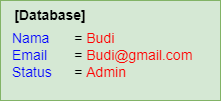
\includegraphics[scale=0.7]{Gambar/config.png}
	\caption{Contoh File Konfigurasi Sederhana} 
	\label{fig:config}
\end{figure}
Pada Gambar \ref{fig:config} merupakan contoh file konfigurasi sederhana. Tulisan ``[Database]'' pada gambar \ref{fig:config} merupakan \textit{section}, untuk tulisan yang berwarna biru merupakan bagian \textit{key}, dan tulisan yang berwarna merah merupakan bagian \textit{value}. Berikut ini penjelasan \textit{key} dan \textit{value} dari Gambar \ref{fig:config}:
\begin{itemize}
	\item Pada file konfigurasi dengan \textit{section} ``[Database]'' memiliki 3 \textit{key} dan \textit{value}.
	\item \textit{Key} pertama adalah ``Nama'' dengan \textit{value} ``Budi''.
	\item \textit{Key} kedua adalah ``Email'' dengan \textit{value} ``Budi@gmail.com''.
	\item \textit{Key} ketiga adalah ``Status'' dengan \textit{value} ``Admin''.
\end{itemize}

\subsection{\textit{Library} Tkinter}
\textit{Library} Tkinter (Tk interface) adalah \textit{library} stadar dari Python untuk membuat aplikasi Python dengan antarmuka yang mudah diprogram. Tk merupakan sebuah fasilitas untuk grafis dan \textit{scripting} yang dikembangkan oleh John Ousterhout {\cite{tkinter}}. Modul yang digunakan dari \textit{library} Tkinter untuk pembuatan program ini adalah tkinter.messagebox. Modul tkinter.messagebox ini berguna untuk memberi suatu informasi mengenai status dari proses dalam menjalankan sebuah program. Berikut ini adalah beberapa fungsi untuk menampilkan status untuk \textit{message box} yang digunakan dalam pembuatan program:
\begin{itemize}
	\item messagebox.showinfo(): Menampilkan informasi yang berguna untuk pengguna. Pada Gambar \ref{fig:infoBox} yang merupakan sebuah contoh tampilan \textit{message box} berupa informasi yang berisi informasi bahwa ``Absensi Berhasil''. 
	\begin{figure}[H]
		\centering
		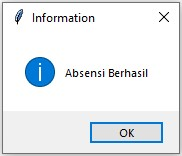
\includegraphics[scale=0.9]{Gambar/infoBox.jpg}
		\caption{Contoh Informasi dari \textit{Message Box}} 
		\label{fig:infoBox}
	\end{figure}
	\item messagebox.showwarning(): Menampilkan sebuah peringatan kepada pengguna.  Pada Gambar \ref{fig:warningBox} yang merupakan sebuah contoh tampilan \textit{message box} berupa \textit{warning} yang berisi peringatan bahwa ``Absensi Gagal!''. 
	\begin{figure}[H]
		\centering
		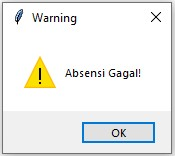
\includegraphics[scale=0.9]{Gambar/warningBox.jpg}
		\caption{Contoh Warning dari \textit{Message Box}} 
		\label{fig:warningBox}
	\end{figure}
\end{itemize}

\subsection{\textit{Library} OS}
\textit{Library} OS adalah modul sistem operasi pada python yang menyediakan cara untuk dapat berinteraksi langsung dengan sistem operasi. Sistem operasi yang dapat melakukan interaksi dengan python adalah windows, linux, dan mac. Berikut ini beberapa fungsi yang dimiliki pada \textit{Library} OS:
\begin{itemize}
	\item os.environ: Melakukan pemetaan terhadap objek yang mewakili \textit{enviroment variable} milik pengguna.
	\item os.getcwd() : Mengembalikan direktori kerja yang digunakan. 
\end{itemize}
